\documentclass[12pt]{article}
\usepackage{chemfig}
\usepackage{carbohydrates}
\usepackage{graphicx}
\usepackage{gensymb}
\usepackage[version=4]{mhchem}
\usepackage{polyglossia}
\usepackage{fontspec}
\usepackage{titlesec}
\usepackage{lettrine}
\usepackage{xcolor}
\usepackage{epigraph, varwidth}
\usepackage{siunitx}
\setlength{\epigraphwidth}{0.8\textwidth}
% sectioning used with \paragraph{at subsubsubsection}
\setcounter{secnumdepth}{4}
\titleformat{\paragraph}
{\normalfont\normalsize\bfseries}{\theparagraph}{1em}{}
\titlespacing*{\paragraph}
{0pt}{3.25ex plus 1ex minus .2ex}{1.5ex plus .2ex}
% sectioning
\setdefaultlanguage{english}
\setotherlanguages{marathi}
\newfontfamily\marathifont[Mapping=velthuis-sanskrit,Script=Devanagari,Language=Marathi]{Shobhika}
\usepackage{soul}
% table with newline in headings
\usepackage{longtable}
\usepackage{makecell}
\renewcommand{\cellalign}{tl}
\renewcommand{\theadalign}{tl}
% table with newline in headings
\usepackage{hyperref}
\hypersetup{
    backref,
    colorlinks=true,
    filecolor=magenta,
    linkcolor=blue,
    urlcolor=violet,
    citecolor=blue,
}
\urlstyle{same}
% new commands
\newcommand{\ctext}[3]{
    \colorbox{#2}{\parbox{0.9\textwidth}{\textcolor{#1}{#3}}}
}
% new commands
% other settings
\setlength{\parindent}{0pt}% Remove paragraph indent
% other settings
\begin{document}
\title{Self-study Notes on OpenStax AP Biology Books and Other Resources}
\author{Kedar Mhaswade}
\date{2020-21}
\maketitle
\def\dev{\edef~{\string~}\textmarathi}
\section{Unit 1: The Chemistry of Life}
\subsection{The Study of Life}
\subsection{The Chemical Foundation of Life}
\subsection{Biological Macromolecules}
\subsubsection{Introduction}
\lettrine[lines=2]{F}{ood provides} the body with the nutrients it needs to survive. Many of these nutrients are ``macro'' or large molecules necessary for and built by living things. They are \emph{necessary} because humans have evolved to use them for survival: 
\begin{itemize}
    \item amino acids in protein for healthy bone and muscle, 
    \item fats to build new cells, store energy, and digest properly, 
    \item carbohydrates to drive all living processes, and
    \item nucleic acids to carry genetic information.
\end{itemize}

Even so, an \emph{imbalance} in our consumption of these macromolecules may lead to health problems. My personal view here is that since all humans are different (however similar they may be) and there are many theories of a general human diet and human feelings are involved in defining what ``health'' means, it is best to spend some time understanding oneself and one's reactions to dietary components. Such a knowledge about oneself is often illusive because humans are very complex multicellular organisms. Whereas macromolecules are absolutely essetial, there are nutrients like vitamins and minerals that have now become equally essential (in much smaller quantities as compared to macromolecules identified above), perhaps not for survival, but to  \emph{manage} health problems and age gracefully.
\subsubsection{Synthesis of Biological Macromolecules}
Biological Macromolecules (BMm's henceforth) are made of atoms of 6 elements: S, P, O, N, C, H. A majority of cell's \emph{dry mass} is made of BMm's. 
\paragraph{Dehydration Synthesis}\label{sec: dehydration synthesis}
BMm's are \emph{polymers} which are chains of \emph{monomers} joined by covalent bonds. A common polymer is the disaccharide \emph{maltose}: \ce{C12H22O11} which is formed when two glucose (\ce{C6H12O6}) molecules combine releasing a water molecule:\\
\ce{2C6H12O11 -> C12H22O11 + H2O}\\

\setchemfig{cram width=2pt}
\schemestart
\chemname
{\chemfig{
([2,0.5]-)([6,0.5]-HO)-[1]([2,0.5]-\ce{CH2OH})([6,0.5]-H)-O-[7]% rightmost C
([2,0.5]-H)([6,0.5,,,red]-OH)<[5] 
([2,0.5]-H)([6,0.5]-OH)-[4,,,,line width=2pt]([2,0.5]-OH)([6,0.5]-)>[3]
}}
{D-Glucose}
\+
\chemname
{\chemfig{
([2,0.5]-)([6,0.5]-HO)-[1]([2,0.5]-\ce{CH2OH})([6,0.5]-H)-O-[7]% rightmost C
([2,0.5]-H)([6,0.5,,,red]-OH)<[5] 
([2,0.5]-H)([6,0.5]-OH)-[4,,,,line width=2pt]([2,0.5]-OH)([6,0.5]-)>[3]
}}
{D-Glucose}
\arrow(.mid east--.mid west)
\schemestop
\vspace{1cm}
\par\medskip
\schemestart
\chemname
{\chemfig{
([2,0.5]-)([6,0.5]-HO)-[1]([2,0.5]-\ce{CH2OH})([6,0.5]-H)-O-[7]% rightmost C left glucose
([2,0.5]-H)([7]-O-[1]
([2,0.5]-H)-[1]([2,0.5]-\ce{CH2OH})([6,0.5]-)-[0]O-[7]
([2,0.5]-H)([6,0.5]-OH)
<[5]
([2,0.5]-H)([6,0.5]-OH)-[4,,,,line width=2pt]([2,0.5]-OH)([6,0.5]-)>[3]
)
<[5]
([2,0.5]-H)([6,0.5]-OH)-[4,,,,line width=2pt]([2,0.5]-OH)([6,0.5]-)>[3]
}}
{Maltose}
\+
\chemname{\chemfig{H_2O}}{Water}
\schemestop

The monomers share electrons as they form covalent bonds. It is called ``dehydration synthesis'' because it literally means formation (of a polymer, in this case) while losing water.

\paragraph{Hydrolysis} \label{sec: hydrolysis}
An almost opposite of \hyperref[sec: dehydration synthesis]{Dehydration Synthesis} is Hydrolysis which literally means separation (-lysis) with water (hydro-). Thus, the energy contained in bonds of polymers is released when they react with water (water is split into hydrogen and hydroxyl ions) and monomers are created.

\ctext{black}{lime}{
    Dehydration Synthesis \emph{requires} energy and releases water to form [polymer] bonds.
}
\par
\ctext{white}{purple}{
    Hydrolysis requires water and \emph{releases} energy stored in [polymer] bonds.
}

\paragraph{Enzymes}
Both these kinds of reaction require enzymes that are \emph{specific} to the BMm's:
\begin{table}[htbp!]
  \begin{center}
    \caption{Enzymes for Hydrolysis of BMm's}
    \label{tab:enzymes-bmms}
    \begin{tabular}{|r|l|} 
      \hline
      \textbf{BMm} & \textbf{Enzymes}\\
      \hline
      Carbohydrates & amylase, sucrase, lactase, or maltase\\
      \hline
      Proteins & pepsin, peptidase, hydrochloric acid\\
      \hline
      Lipids & lipase\\
      \hline
    \end{tabular}
  \end{center}
\end{table}


\ctext{black}{teal}{
    \small{
        We wonder how life formed on Earth. In 1953, Stanley Miller and Harold Urey developed an apparatus to model early conditions on earth. They wanted to test if \emph{organic molecules could form from inorganic precursors believed to exist very early in Earth’s history}. They used boiling water to mimic early Earth’s oceans. Steam from the “ocean” combined with methane, ammonia, and hydrogen gases from the early Earth’s atmosphere and was exposed to electrical sparks to act as lightning. As the gas mixture cooled and condensed, \emph{it was found to contain organic compounds, such as amino acids and nucleotides}. According to the \textbf{abiogenesis theory} (the original evolution of life or living organisms from inorganic or inanimate substances), these organic molecules came together to form the earliest form of life about 3.5 billion years ago.
   }
}
\subsubsection{Carbohydrates}
The \href{https://en.wikipedia.org/wiki/Carbohydrate}{Wikipedia page on Carbohydrates} is comprehensive. A few things to know about carbohydrates:
\begin{itemize}
    \item A carbohydrate consists of carbon, hydrogen, and oxygen atoms, usually (\emph{but not always}) with a 2:1 hydrogen-oxygen atom ratio and the empirical formula \ce{C_m(H2O)_n}.
    \item In biochemistry, the term \emph{carbohydrates} is synonymous with the term \emph{saccharides} which contain sugars, starch, and cellulose. 
    \item Four main groups (of these, the first two are commonly referred to as sugars): 
        \begin{enumerate}
            \item monosaccharides (simple sugars: \ce{(CH2O)_n}): Simplest of carbohydrates. \textbf{They cannot be hydrolyzed into simpler compounds}. Common examples: glyceraldehyde, ribose, glucose, fructose, and galactose.
            \item disaccharides: Formed when two monosaccharide molecules are joined with the (covalent) glycosidic bonds. Common examples: sucrose, lactose, and maltose.
            \item oligosaccharides: Consist of a few to several monosaccharide molecules (as a rule of thumb: 3 to 10). Common examples: glycolipids.
            \item polysaccharides: These long chains of monosaccharide molecules (as a rule of thumb: more than 10) are the most abundant carbohydrates in human food. Two main types:
            \begin{enumerate}
                \item Storage polysaccharides: starch, glycogen, and galactogen.
                \item Structural polysaccharides: cellulose and chitin.
            \end{enumerate}
        \end{enumerate}
    \item Common names -- fructose (a monosaccharide): \emph{fruit sugar}, glucose (a monosaccharide): \emph{starch sugar}, sucrose (a disaccharide): \emph{cane} or \emph{beet sugar}, lactose (a disaccharide): \emph{milk sugar}.
    \item 
\end{itemize}
\paragraph{Monosaccharides}
Monosaccharides are the simplest form of sugar. They cannot be further \hyperref[sec: hydrolysis]{\emph{hydrolyzed}} to simpler chemical compounds. They are classified according to number of carbon atoms. They are also classified according to the functional group they contain. Based on the number of carbon atoms they are classified as triose, tetrose, pentose, hexose and so on. Based on the functional group, they are classified as either aldose (aldehyde group: \ce{R-CHO}) or ketose (ketone group: \ce{R-C=O-R$^{'}$}).
\subsubsection{Lipids}
\subsubsection{Proteins}
Proteins are long chains (sequences) of amino acids. There are 20 common amino acids. An amino acid is a monomer; itcontains an amino group (\ce{-NH2}), a carboxyl group (\ce{-COOH}), and a variable group. Suppose that a certain protein is a sequence of \textbf{500} amino acids, then since we have 20 choices to pick from for each of the 500 amino acid molecules, there are $20^{500}$ (a huge number!) choices to make the protein. The following diagram shows a simple protein that is a sequence of just 8 amino acids: 
\begin{table}[htbp!]
  \begin{center}
    \caption{An Example Protein: a Sequence of 8 Amino Acids}
    \label{tab: simple protein}
    \begin{tabular}{|c|c|c|c|c|c|c|c|} 
      \hline
        AA-15 &
        AA-02 &
        AA-20 &
        AA-11 &
        AA-03 &
        AA-10 &
        AA-07 &
        AA-18 \\
        \hline
    \end{tabular}
  \end{center}
\end{table}
This hypothetical case of all proteins being a sequence of just 8 amino acids would yield 
$20^8=25,600,000,000$ different proteins. Table \ref{tab: simple protein} just shows one possible arrangement. Although amino acids have names, we have simply referred to them as AA-1 to AA-20 in that example. In nature, proteins are arbitrarily long sequences of amino acids.

In proteins, each amino acid molecule is linked to the next by a \emph{peptide bond} formed by dehydration synthesis (not unlike the formation of polysaccharides from monosaccharides). This makes protein a \emph{polypeptide}. Proteins are really the workhorses in organisms. They carry out the following functions:
\begin{itemize}
    \item Act as enzymes that catalyze chemical reactions
    \item Provide structural support (along with cellulose which is available only in plants)
    \item Regulate the passage of substances across the cell membrane (even viruses and other pathogens may \emph{attach} to proteins to enter cells)
    \item Help protect against (infectious) diseases (by participating in antibody creation)
    \item Communicate with other cells; receptors which are proteins receive and transduce \emph{signals}
\end{itemize}

Characteristic property of proteins is their \emph{folding} or three-dimensional structure. Predicting Protein Folding from its linear structure is very useful for research and it is also a major computational problem. Recently, AI techniques have been used for this purpose \cite{alphafold}. Protein Folding occurs at four levels:
\begin{enumerate}
    \item Primary: Decides the unique (linear) sequence of amino acids; a single amino acid change in a protein can alter its structure and function
    \item Secondary: Consists of the local folding of the polypeptide by hydrogen bond formation leading to $\alpha$ helix and $\beta$ pleated sheet \emph{conformations}
    \item Tertiary: Various interactions give rise to the three-dimensional structure
    \item Quaternary: May be formed from several polypeptide interactions
\end{enumerate}

Proteins may stop functioning when they are \emph{denatured} which depends upon environmental conditions like temperature and pH.

\paragraph{Types and Functions of Proteins}
Each cell may contain thousands of proteins. Their structures, like their function, may vary greatly. 

\begin{table}[htbp!]
  \begin{center}
    \caption{Types and Functions of Proteins}
    \label{tab: protein-types-functions}
    \begin{tabular}{|c|c|c|} 
      \hline
        \thead{\textbf{Type of Protein}} & 
        \thead{\textbf{Examples}} & 
        \thead{\textbf{Functions}}\\
      \hline
        Digestive Enzymes & 
        \makecell{Amylase, lipase, \\pepsin, and trypsin} &
        \makecell{
        Help in digestion of\\ food by catabolizing \\
        nutrients into monomeric units}\\
      \hline
        Transport & 
        \makecell{Hemoglobin, albumin} &
        \makecell{
        Carry substances in blood\\ or lymph throughout\\
        the body}\\
      \hline
        Structural & 
        \makecell{Actin, tubulin, keratin} &
        \makecell{
            Construct different structures\\ like e.g. cytoskeleton}\\
      \hline
        Hormone & 
        \makecell{Insulin, thyroxine} &
        \makecell{
            Coordinate activities in \\ different body systems by \\
        participating in cell signaling}\\
        \hline
        Defense & 
        \makecell{Immunoglobulins} &
        \makecell{
            Protect the body \\ from pathogens }\\
        \hline
        Contractile & 
        \makecell{Actin, myosin} &
        \makecell{
            Effect muscle contraction}\\
        \hline
        Storage & 
        \makecell{Legume storing proteins, albumin} &
        \makecell{
            Provide nourishment \\ in early development\\
        of the embryo and the seedling}\\
        \hline
    \end{tabular}
  \end{center}
\end{table}

\paragraph{Amino Acids}
Amino acids are the monomers that make up proteins. Each amino acid has the same fundamental structure, which consists of a central carbon atom, also known as the alpha ($\alpha$) carbon, bonded to an amino group (\ce{NH2}), a carboxyl group (\ce{COOH}), and to a hydrogen atom. Every amino acid also has another atom or group of atoms bonded to the central atom known as the R group.

\begin{figure}[h!]
    \centering
    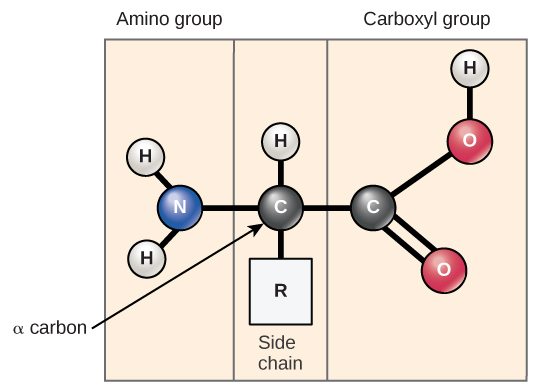
\includegraphics[width=0.5\linewidth]{openstax-protein-general-structure.jpg}
    \caption{The General Structure of a Protein (From OpenStax)}
    \label{fig: protein}
\end{figure}

Amino acids can be looked upon as \ce{R-COOH}. Since the carboxyl group makes a molecule acidic (it tends to readily lose the hydrogen atom or proton and form the \ce{COO-} ion in a phenomenon called deprotonation).

Twenty common amino acids are found in proteins. Nine of these are considered \emph{essential} since they cannot be synthesized in the body and have to be obtained from the diet. For each amino acid the R-group (the side chain) is different.

Wikipedia reports that the proteinogenic amino acids are amino acids that are incorporated biosynthetically into proteins during translation. The word ``proteinogenic" means "protein creating". Throughout known life, there are 22 genetically encoded (proteinogenic) amino acids, 20 in the standard genetic code and an additional 2 that can be incorporated by special translation mechanisms.

\subsubsection{Nucleic Acids}
Nucleic acids (DNA and RNA) contain phosphorus in addition to C, H, O, and N. \textbf{Conserved through evolution in all organisms, nucleic acids store and transmit hereditary information}. A cell (nucleus) contains DNA spread across various chromosomes. In humans, each chromosome comes as a \emph{pair}, that is, if we numbered chromosomes 1, 2, $\dots$, then humans have a pair of each number. A chromosome is, in turn, a \href{https://biology.stackexchange.com/a/996/63085}{pair of distinct DNA molecules} connected by hydrogen bonds.


\ctext{white}{purple}{
    1 chromosome = 2 DNA molecules
}

All matter is made of atoms and molecules and bonds between them. Nucleic acids are polymers. One molecule of a nucleic acid is made of several other molecules. Think of this or any other polymer as a hierarchical structure that becomes progressively bigger and more complex.

One molecule of a nucleic acid could be made of tens of thousands of the monomeric \emph{Nucleotide} molecules. Each nucleotide molecule in turn is made of 
\begin{itemize}
    \item one molecule of \emph{Nucleoside} which is made of
        \begin{itemize}
            \item one molecule of a nitrogenous base (Nucleobase) and
            \item one molecule of a pentose sugar (ribose in RNA and deoxy-ribose in DNA)
        \end{itemize}
    \item one, two, or three molecules of a phosphate 
\end{itemize}

The nucleotide molecules are held together by phosphodiester bonds. A \emph{nucleoside} is either
\begin{itemize}
    \item Adenine (both DNA and RNA),
    \item Cytosine (both DNA and RNA),
    \item Guanine, (both DNA and RNA),
    \item Thymine (only DNA), or
    \item Uracil (only RNA)
\end{itemize}

There are differences between RNA and DNA. There is only one form of DNA, whereas RNA has various forms: messenger RNA (mRNA), transfer RNA (tRNA), ribosomal RNA (rRNA), micro RNA (miRNA). In DNA, there is its signature \emph{double helical structure}. 


\paragraph{The Central Dogma of Molecular Biology}
\label{para: central-dogma}
\epigraph
{
    \dots Once the `information' has passed into protein \textit{it cannot get out again}. In more detail, the transfer of information from nucleic acid to nucleic acid, or from nucleic acid to protein may be possible, but transfer from protein to protein, or from protein to nucleic acid is impossible. \textbf{Information means here the precise determination of sequence, either of bases in the nucleic acid or of amino acid residues in the protein}.
}
{
    -- As stated by Francis Crick \cite{the-central-dogma}
}

\paragraph{DNA and RNA}
Both DNA and RNA are, of course, examples of a \emph{nucleic acid}. This \emph{genetic material} has different functions. DNA, which stands for the \emph{Deoxyribose Nucleic Acid} has, one oxygen atom \textbf{less than} (per repetitive nucleotide unit) RNA, which stands for \emph{RiboNucleic Acid}. Figures \ref{fig: dna} and \ref{fig: rna} show their chemical structures.

\begin{figure}[ht!]
    \centering
    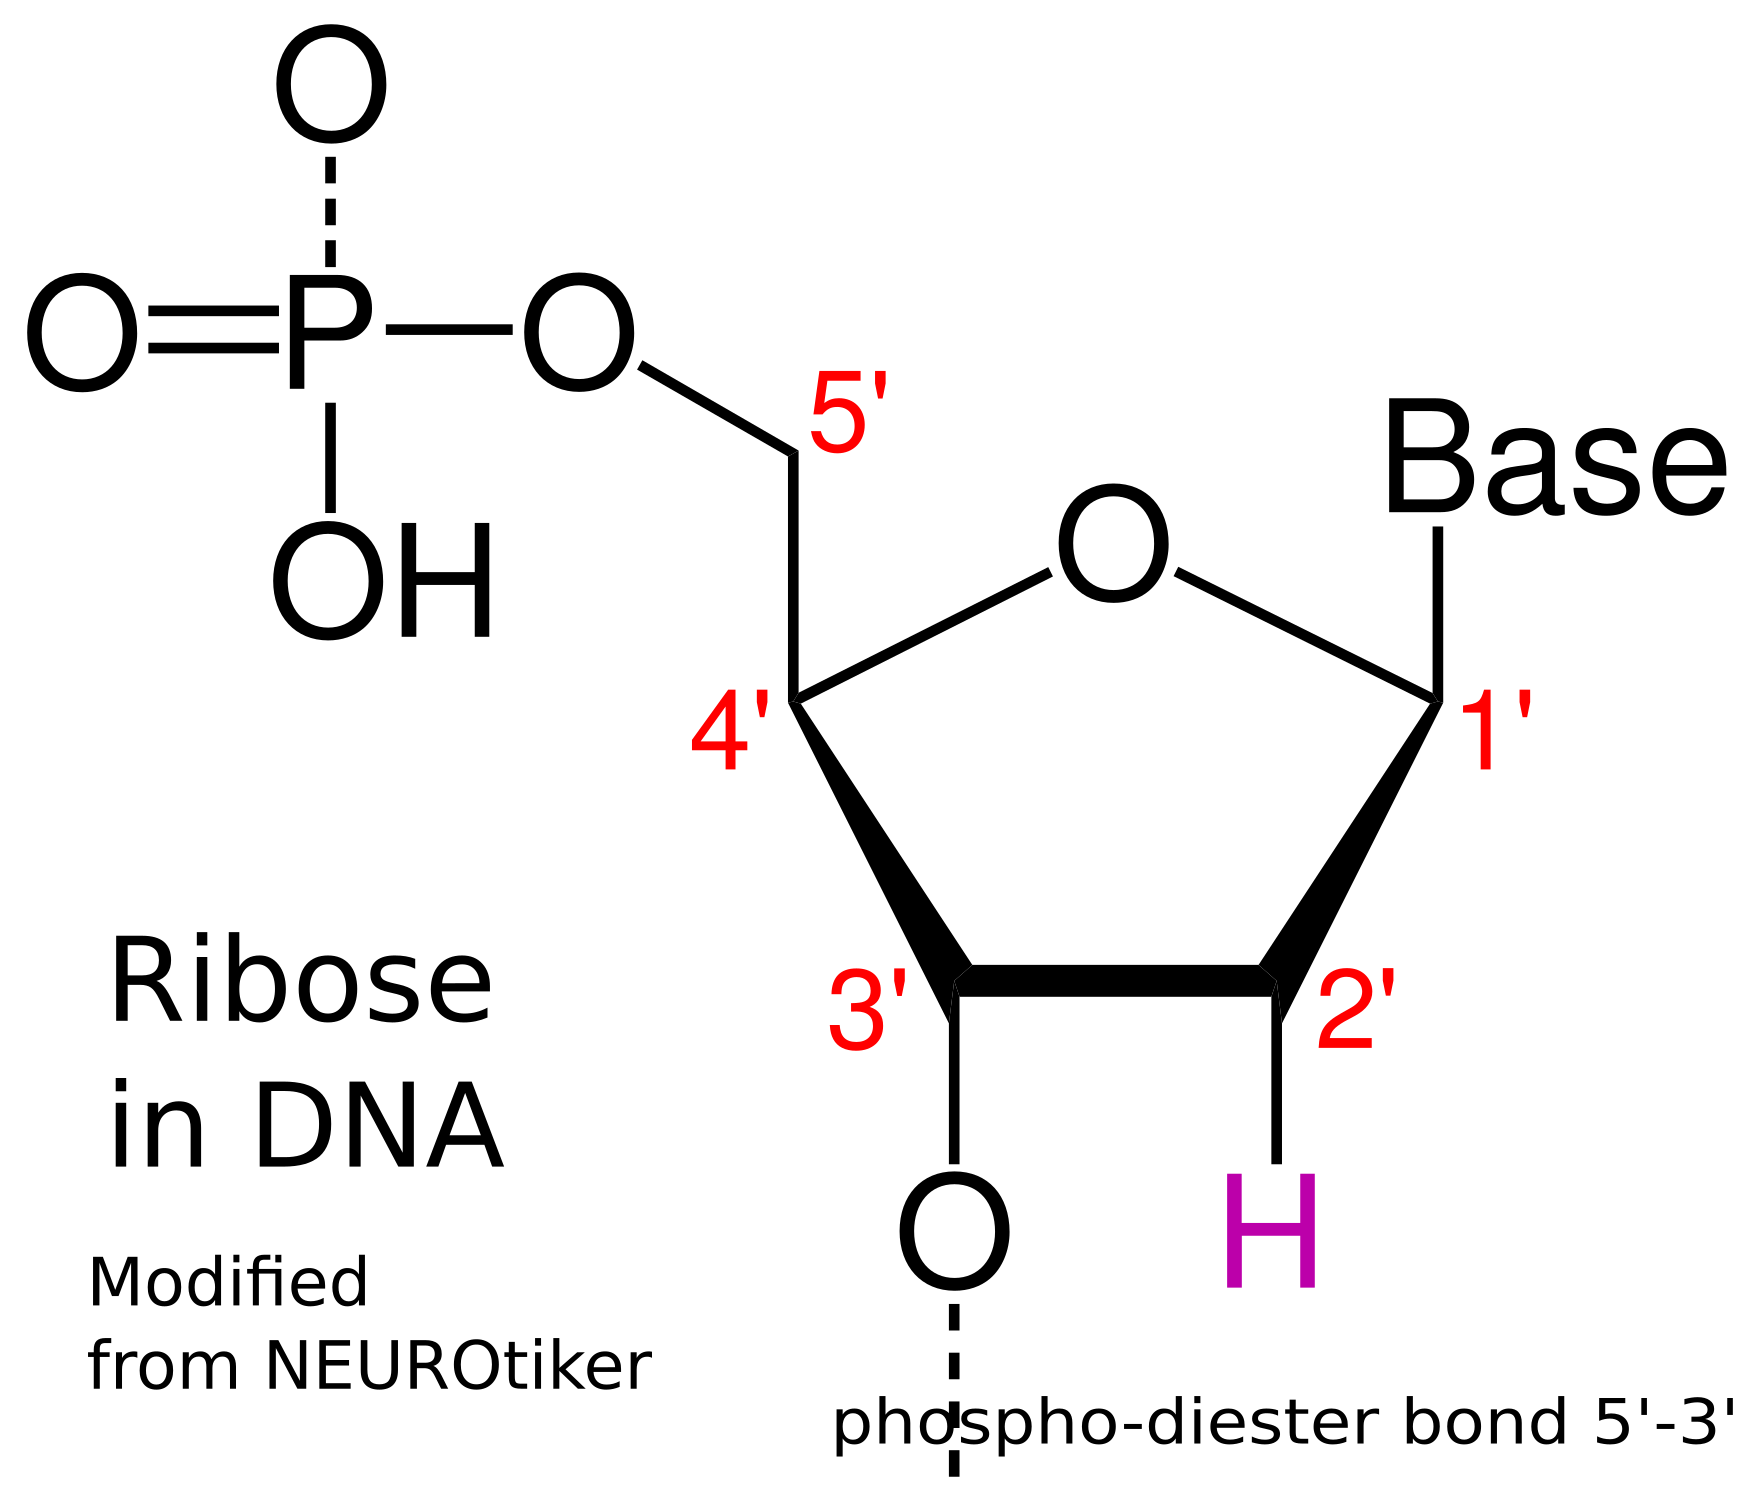
\includegraphics[width=0.5\linewidth]{dna-ribose-numbering-std-notation.png}
    \caption{DNA}
    \label{fig: dna}
\end{figure}

\begin{figure}[ht!]
    \centering
    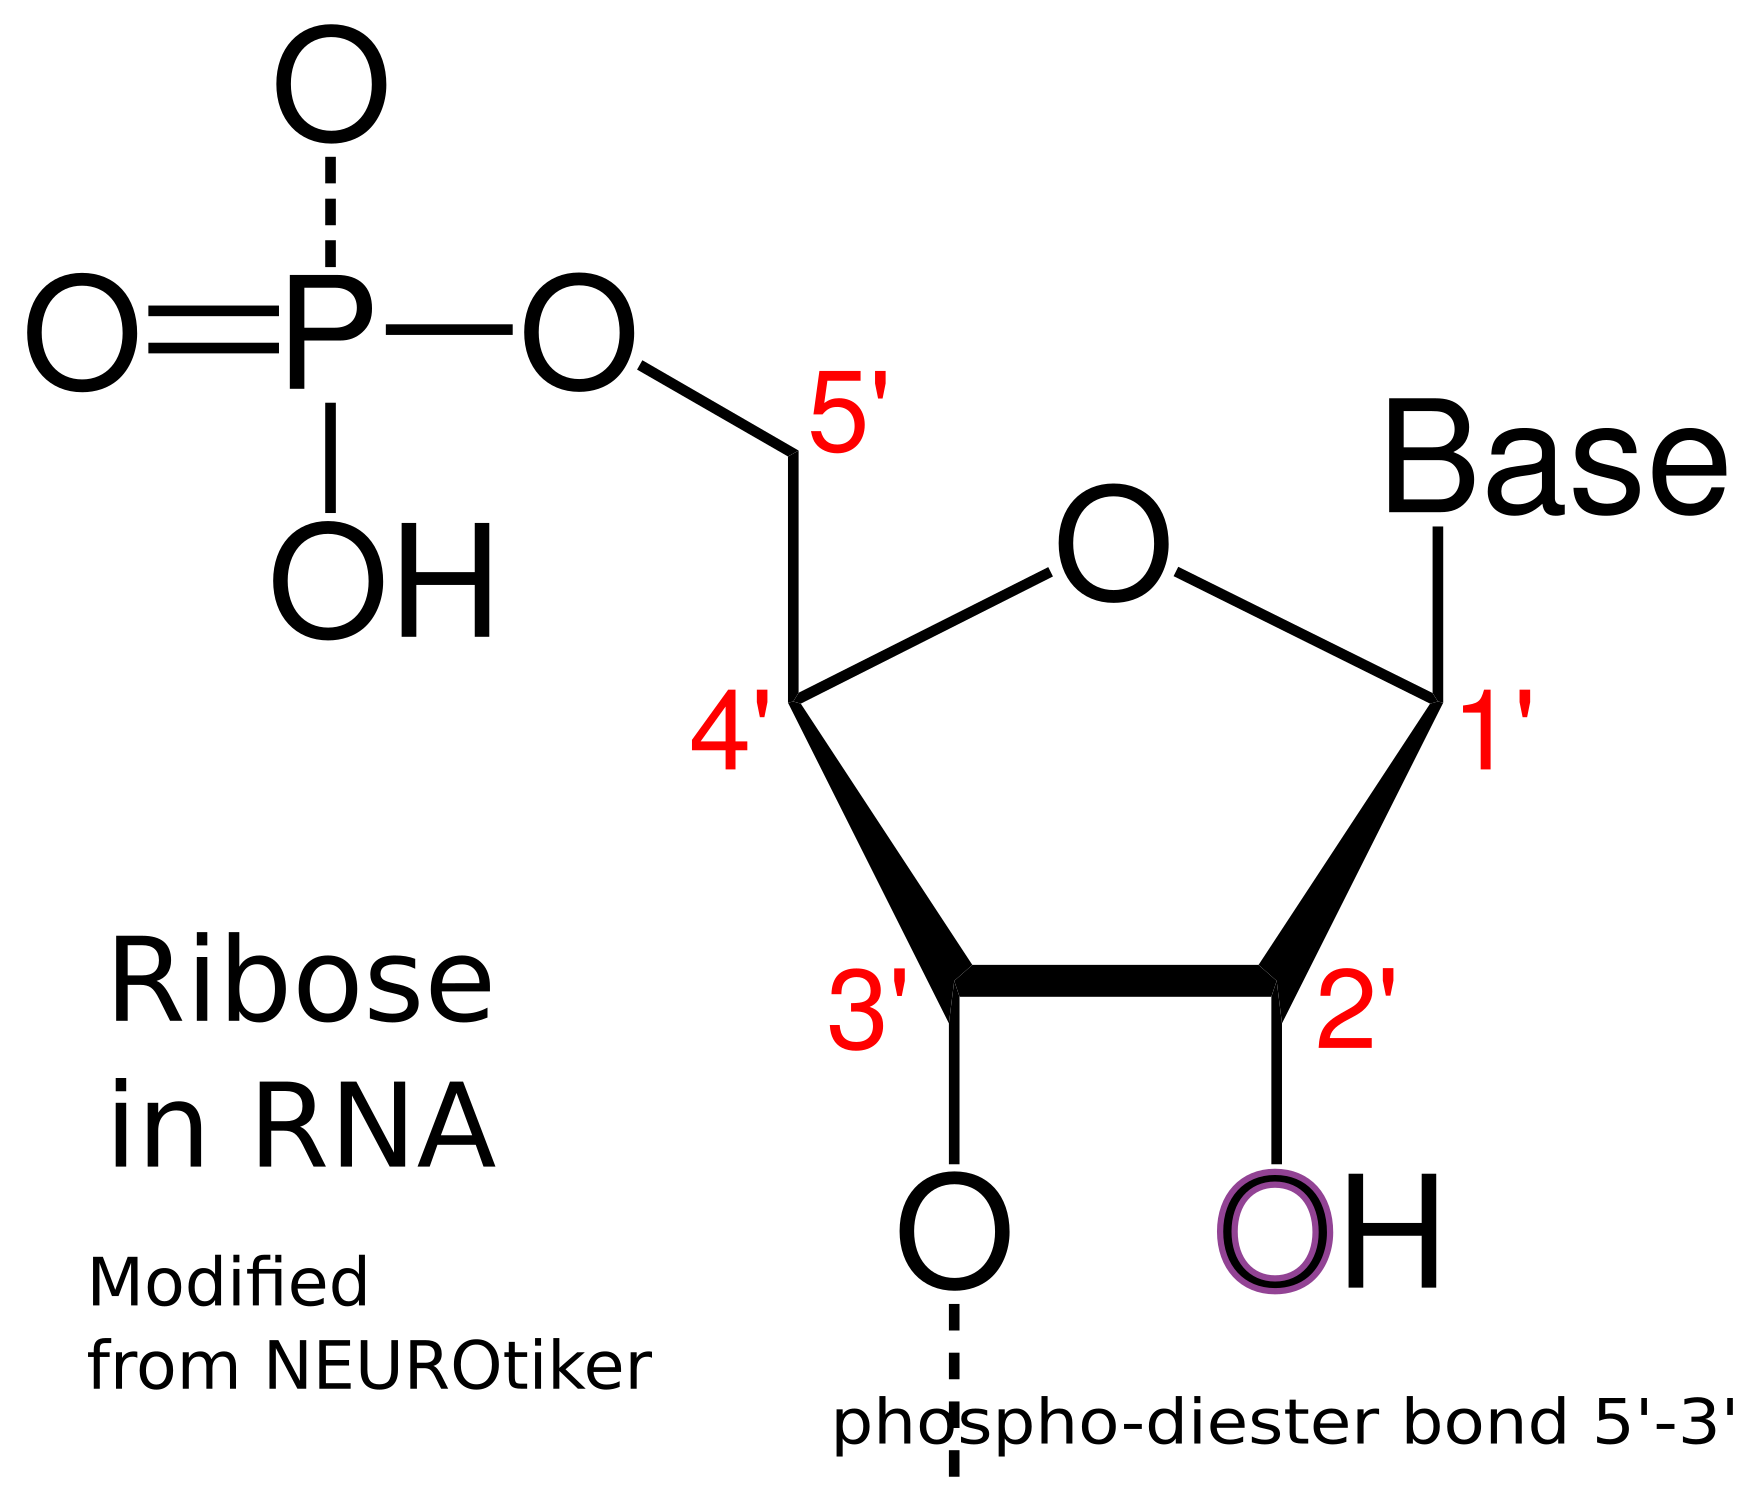
\includegraphics[width=0.5\linewidth]{rna-ribose-numbering-std-notation.png}
    \caption{RNA}
    \label{fig: rna}
\end{figure}

The \emph{strand} of several nucleotides in DNA looks like Figure \ref{fig: dna-strand}.

\begin{figure}[ht!]
    \centering
    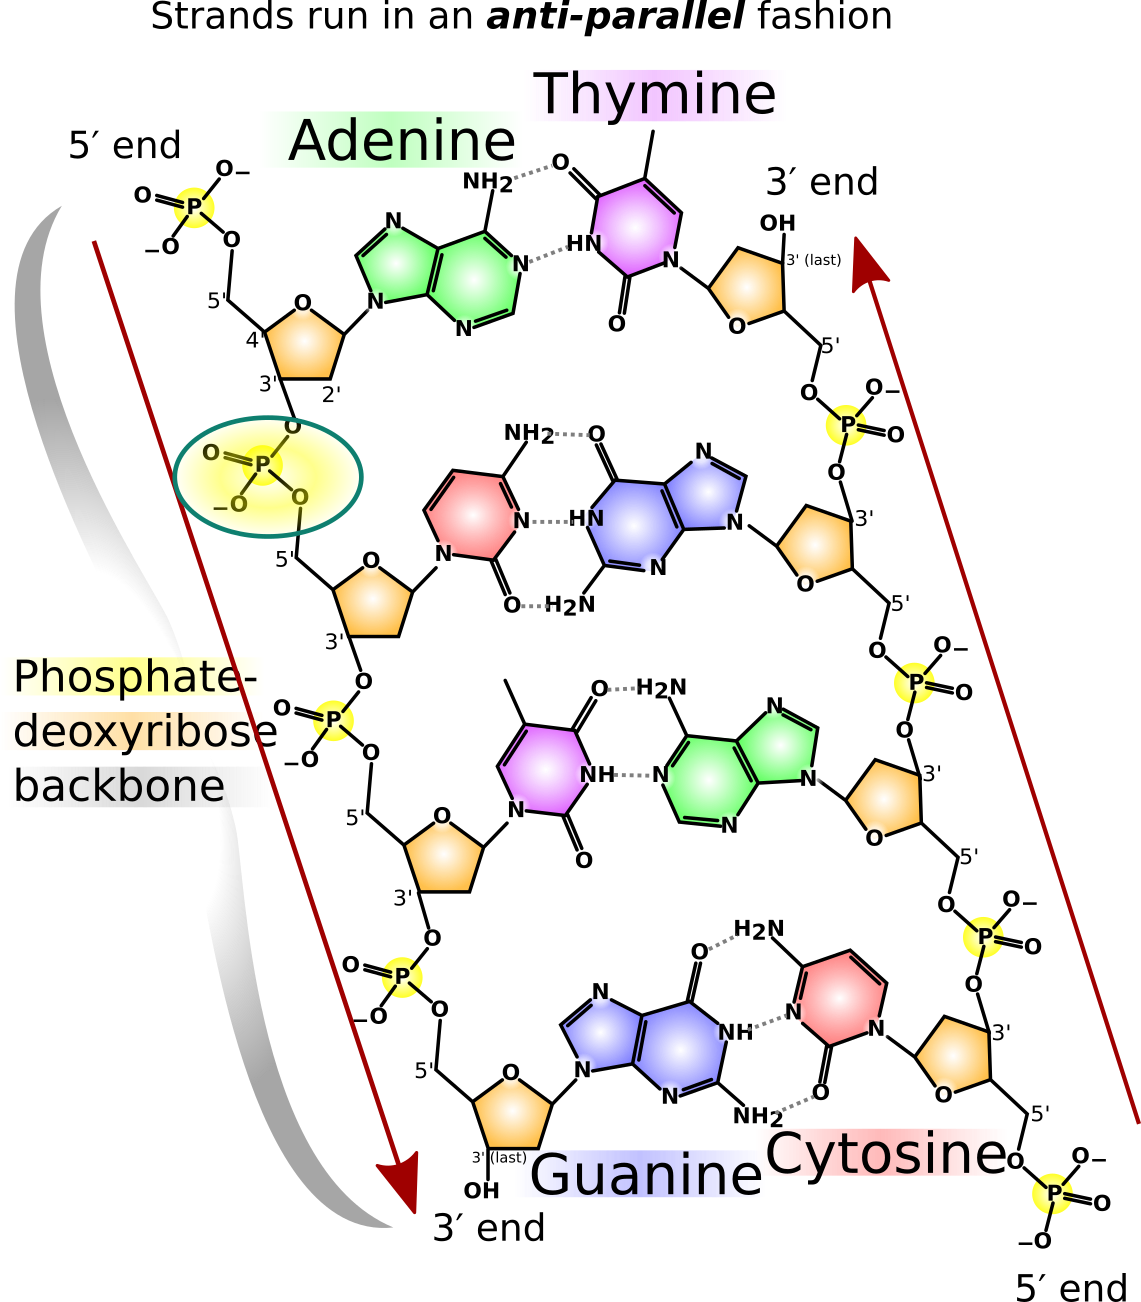
\includegraphics[width=0.6\linewidth]{DNA_chemical_structure-madprime.png}
    \caption{A DNA Strand}
    \label{fig: dna-strand}
\end{figure}


The structures of nucleic acids reveal that they have nitrogenous base and phosphate. You may wonder why it is called an acid if it has a nitrogenous \emph{base}. Looking at the \emph{phosphodiester bonds} between the nucleotide molecules in a DNA or RNA molecule \href{https://biology.stackexchange.com/questions/3864/dna-as-an-acid}{should help decide}. See Figure \ref{fig: dna-strand}. The phosphate group (blurred yellow oval in Figure \ref{fig: dna-strand}) is similar to the phosphoric acid (\ce{H3PO4}) molecule which has 3 hydrogen atoms. In DNA or RNA nucleotide chain, the two hydrogen atoms (from the phosphoric acid) are replaced by (the 5' and the 3') carbon atoms on the ribose sugar molecule. This makes the remaining hydrogen extremely reactive and it is lost rather easily under neutral conditions. As the Figure \ref{fig: dna-strand} shows, the oxygen on the phosphate group assumes a negative charge because the molecule literally gets \emph{deprotonated}. This makes the DNA or RNA molecule acidic in nature as a whole in spite of the fact that there are a lot of nitrogenous base molecules in it\footnote{DNA is \emph{double stranded} and there are separate hydrogen bonds between the nitrogenous bases (purines and pyrimidines) as well.}.

The nitrogenous bases, important components of nucleotides, are organic molecules and are so named because they contain carbon and nitrogen. They are bases because they contain an amino group that has the \textbf{potential of binding an extra hydrogen, thus decreasing the hydrogen ion concentration in its environment, making it more basic}. Each nucleotide in DNA contains one of four possible nitrogenous bases: adenine (A), guanine (G) cytosine (C), and thymine (T).

Adenine and guanine are classified as purines. The primary structure of a purine is two carbon-nitrogen rings. Cytosine, thymine, and uracil are classified as pyrimidines which have a single carbon-nitrogen ring as their primary structure. Each of these basic carbon-nitrogen rings has different functional groups attached to it. In molecular biology shorthand, the nitrogenous bases are simply known by their symbols A, T, G, C, and U. DNA contains A, T, G, and C whereas RNA contains A, U, G, and C.

The pentose sugar in DNA is deoxyribose, and in RNA, the sugar is ribose. The difference between the sugars is the presence of the hydroxyl group on the second carbon of the ribose (Figure \ref{fig: rna}) and hydrogen on the second carbon of the deoxyribose (Figure \ref{fig: dna}). The carbon atoms of the sugar molecule are numbered as 1', 2', 3', 4', and 5' (1' is read ``one prime"). The phosphate residue is attached to the hydroxyl group of the 5' carbon of one sugar and the hydroxyl group of the 3' carbon of the sugar of the next nucleotide, which forms a 5'–3' phosphodiester linkage. The phosphodiester linkage is not formed by simple dehydration reaction like the other linkages connecting monomers in macromolecules: its formation involves the removal of two phosphate groups. A polynucleotide may have thousands of such phosphodiester linkages.

\paragraph{DNA Double-Helix Structure}
DNA has a double-helix structure. The sugar and phosphate lie on the outside of the helix, forming the backbone of the DNA. The nitrogenous bases are stacked in the interior, like the steps of a staircase, in pairs; the pairs are bound to each other by hydrogen bonds (See Figure \ref{fig: dna-strand}). Every base pair in the double helix is separated from the next base pair by\footnote{Charles Mallery \cite{mallery} reports that one full turn of the helix is about 3.4 nanometers, or 10 base pairs long.} 0.34 nm. The two strands of the helix run in opposite directions, meaning that the 5' carbon end of one strand will face the 3' carbon end of its matching strand. (This is referred to as \emph{antiparallel} orientation and is important to DNA replication and in many nucleic acid interactions.)

Erwin Chargaff studied many species for the \emph{amount} of purines and pyrimidines their cells have. 

\epigraph{
    Chargaff's rules state that DNA from any species of any organism should have a 1:1 stoichiometric ratio (base pair rule) of pyrimidine and purine bases and, more specifically, that the amount of guanine should be equal to cytosine and the amount of adenine should be equal to thymine. This pattern is found in both strands of the DNA. They were discovered by Austrian-born chemist Erwin Chargaff in the late 1940s.
}{
    \textit{Wikipedia entry on Chargaff's rules}
}

Mallery \cite{mallery} states the rules thus:
\begin{enumerate}
    \item A with T: the purine adenine (A) always pairs with the pyrimidine thymine (T)
    \item C with G:  the pyrimidine cytosine (C) always pairs with the purine guanine (G)
\end{enumerate}

This is consistent with there not being enough space (20 \si{\angstrom}) for two purines to fit within the helix and too much space for two pyrimidines to get close enough to each other to form hydrogen bonds between them.

But why not A with C and G with T?

The answer: only with A and T and with C and G are there opportunities to establish hydrogen bonds between them (\emph{two} between A and T; \emph{three} between C and G). The ability to form hydrogen bonds makes the base pairs structurally more stable.

Like in the case of any scientific discovery that becomes an accepted fact, one should see Chargaff's findings in the light of the prevalent scientific understanding at the time. Although Chargaff was \emph{in the vicinity} of making the discovery that DNA has a \emph{double helical} structure, he was not able to do it. This is an interesting example of how creativity\footnote{Of course, several other factors contribute to a discovery and its acceptance by the scientific community.} is illusive in a scientific endeavor: 
\epigraph{
    Our conversation covered many topics. Erwin Chargaff's name came
up and Francis found it strange that Chargaff did not discover base-pairing
in the light of his observations on the base ratios in DNA. However, \emph{this may be more surprising in hindsight}. Just looking at the data, there is much fluctuation, about 10 percent, about the 1 to 1 ratios. So \emph{even recognizing and suggesting the 1 to 1 ratio was a sharp observation}. Francis then added that Chargaff's mind might have not wandered toward pairing
because he, that is, Chargaff \emph{was thinking in terms of one chain rather than two}. In a single chain, nothing would prompt one's thinking toward pairing. Once you know that two chains need be considered, pairing enters
one's thinking more naturally. Francis seemed careful not to use the word
helix at this point, as if placing himself into Chargaff's position. Even if Chargaff was thinking about the significance of the 1 to 1 ratios, about
the possible meaning of such a ratio in a nucleotide chain, it's not surprising that nothing suggested itself for a reasonable solution.
}
{
    -- \textit{Francis Crick Interview by Hargittai and Hargittai \cite{ih-mh} (emphasis mine)}
}
\paragraph{RNA}
Ribonucleic acid, or RNA, is mainly involved in the \emph{process of protein synthesis under the direction of DNA}. RNA is usually single-stranded and is made of ribonucleotides that are linked by phosphodiester bonds. A ribonucleotide in the RNA chain contains ribose (the pentose sugar), one of the four nitrogenous bases (A, \textbf{U}, G, and C), and the phosphate group.

There are four major \emph{functional} types of RNA:
\begin{enumerate}
    \item messenger RNA (mRNA) : literally \emph{carries} the message or the information from DNA; its sequence is complementary to the DNA from which it is copied.
    \item ribosomal RNA (rRNA): a constituent of the ribosomes that binds the mRNA. 
    \item transfer RNA (tRNA)a: a small RNA (70-90 nucleotides) that \emph{transfers} correct amino acid to be inserted into the polypeptide chain that is the protein that an expressed gene encodes. 
    \item mircroRNA (miRNA): the smallest RNA that regulates the \emph{gene expression}.
\end{enumerate}

We stated the \hyperref[para: central-dogma]{\emph{central dogma}} above. It appears to be true of eukaryotes although there are exceptions. Not everyone agrees with the assertion that information cannot come out of proteins. In fact, Eugene Koonin states the following in a Springer Nature article (\cite{koonin}):
\epigraph{
    Central Dogma of molecular biology is invalid as an `absolute' principle: transfer of information from proteins (and specifically from protein sequences) to the genome does exist. This is not to deny that the Central Dogma does capture the principal route of information transfer in biology: the main flow information does follow the path in Figure 1 [DNA $\rightarrow$ RNA $\rightarrow$ protein], and elaborate mechanisms ensuring acceptable fidelity operate on each step. And, there is a major discontinuity between the levels of RNA and protein because during translation because the coupling of amino acids with the cognate tRNAs does not involve direct recognition but rather requires dedicated enzymes, aminoacyl-tRNA synthetases, that recognize and connect the partners. The opposite direction of information flow, from proteins to the genome, is asymmetrical (not a simple reversion), much more modest quantitatively and intrinsically stochastic but nevertheless appears to be important in evolution.
}
{
    -- \textit{Eugene Koonin} \cite{koonin}}
\section{Unit 2: The Cell}
\subsection{Cell Structure}
\paragraph{Introduction}
Cells are the fundamental building blocks of all organisms. There are, of course, many kinds of cell and each kind of cell has a \emph{specific} function to perform. There's tremendous variety of functions that cells perform and the organisms that they create are also diverse (e.g. sponges, bacteria, fungi, plants, animals) in nature. Even so, many cells share a few fundamental characteristics.

A cell's development and growth to perform its eventual tasks is called its ``specialization''. In humans, before a cell develops into its specialized type, it is called a \emph{stem cell}. Thus, stem cells do not undergo changes involved in specialization. Stem cells are called \emph{pluripotent} (that means they are capable of giving rise to several different cell types). There is a great potential in stem cell research to address human illnesses.
\subsubsection{Studying Cells}
\ctext{red}{white}{
    Cells of a kind --- form $\rightarrow$ Tissue --- combine to form $\rightarrow$ Organ (e.g. stomach, heart, or brain) --- make up $\rightarrow$ Organ System(s) (e.g. digestive system, endocrine system) --- work together to form $\rightarrow$ an Organism.
}
\subsubsection{Prokaryotic Cells}
\subsubsection{Eukaryotic Cells}
\subsubsection{The Endomembrane System and Proteins}
\subsubsection{Cytoskeleton}
\subsubsection{Connections between Cells and Cellular Activities}


\subsection{Structure and Function of Plasma Membranes}
\paragraph{Introduction}
The plasma membrane (the PM, henceforth), which is also called the cell membrane, has many functions; but, the most basic one is to \emph{define the borders} and \emph{act as gatekeeper} for the cell.

The PM is a selectively permeable membrane that allows only certain molecules to freely enter cells. Other molecules may require assistance. A striking example of this is the (membrane) protein called NPC1 (\href{https://en.wikipedia.org/wiki/NPC1}{Niemann-Pick Type C1}) which mediates the intracellular cholesterol trafficking in mammals. NPC1 is therefore called a \emph{cholesterol transporter}. A mutation in the NPC1 gene (that encodes the NPC1 protein) may prevent the entry of cholesterol into cells that results in cholesterol accumulation in intercellular space. But this problem may be a boon in disguise because if such an organism is infected with the Ebola virus, since the NPC1 protein's cholesterol transportation is impared, its cells are impervious to the virus even when it binds with NPC1.

\subsection{Metabolism}
\subsubsection{ATP: Adenosine Tri-Phospate}
\begin{itemize}
    \item Even exergonic reactions (those that \textit{release} energy) require a small amount of
        \textit{activation energy} to proceed.
    \item Products of endergonic reactions (those that \textit{require} energy input) have
        more energy than that of their reactants. Where does the cell provide this energy from?
    \item ATP is the molecule that provides the energy required for the endergonic reactions 
        as well as the small activation energy required for the exergonic reactions.
    \item ATP is a \textit{relatively} simple molecule: C\textsubscript{10}H\textsubscript{16}N\textsubscript{5}O\textsubscript{13}P\textsubscript{3} %$C_{10}H_{16}N_{5}O_{13}P_{3}$
        \begin{itemize}
            \item It has adenosine bound to three phosphate groups that are named alpha- (closest to ribose), beta-, and gamma-phosphate (farthest from ribose).
            \item Adenosine is a \textit{nucleoside}---a compound commonly found in DNA or RNA, consisting of a purine or pyrimidine base linked to a sugar.
        \end{itemize}
    \item ATP \textit{hydrolyzes} to ADP (Adenosine Di-Phosphate) and inorganic phosphate. Regeneration of ATP requires energy to be supplied. Thus, hydrolysis of ATP is reversible: \\
        \schemestart ATP + H\textsubscript{2}O\arrow{<=>}ADP + P\textsubscript{i} + free energy\schemestop\par
    \item Cellular conditions differ from standard conditions. In cellular conditions, the $\Delta G$ (change in Gibbs free energy) of ATP's hydrolysis is -57 kJ/mol = -14 kcal/mol.
\end{itemize}


\subsection{Cellular Respiration}
\paragraph{Introduction}
Energy enters an organism’s body in one form and is converted into another form that can fuel the organism’s life functions. In the process of photosynthesis, plants and other photosynthetic producers take in energy in the form of light (solar energy) and convert it into chemical energy, glucose, which stores this energy in its chemical bonds. Then, a series of metabolic pathways, collectively called cellular respiration, extract the energy from the carbon–carbon bonds of glucose and convert it into a form that all living things can use—both producers, such as plants, and consumers, such as animals.
\subsubsection{Energy in Living Systems}
\subsubsection{Glycolysis}
\subsubsection{Oxidation of Pyruvate and the Citric Acid Cycle}
\subsubsection{Oxidative Phosphorylation}
\subsubsection{Metabolism without Oxygen}
\subsubsection{Connections of Carbohydrate, Protein, and Lipid Metabolic Pathways}
\subsubsection{Regulation of Cellular Respiration}
\subsection{Photosynthesis}
\emph{Many organisms} access stored energy by \emph{eating} or \emph{ingesting (consuming)} other organisms: \textmarathi{jiivo jiivasya jiivanam|}. All of this energy can be traced back to photosynthesis.
\subsubsection{Overview}
Photosynthesis is the \emph{only} biological process that can capture the energy in sunlight and convert it into the energy stored in the covalent bonds of sugar molecules. Additionally, it acts as a source of oxygen necessary for \emph{many} living organisms.

\emph{Photoautotrophs} (organisms that use light to synthesize their own food) such as plants, algae(\textmarathi{\dev aljii}), and cyanobacteria are the only ones that can perform photosynthesis.

\emph{Chemoautotrophs} (organisms that use energy stored in inorganic molecules, and not sunlight, to synthesize their own food) found in deep sea represent another class of \emph{autotrophs}.

Animals, fungi, and most other bacteria are termed \emph{Heterotrophs} because they have to rely on the sugars produced by Photoautotrophs.

\paragraph{Main Structures and Summary}
Photosynthesis is a multi-step process that requires
\begin{enumerate}
    \item Specific wavelengths of visible sunlight and
    \item Carbon dioxide (low in energy) and water as substrates.
\end{enumerate}
It 
\begin{enumerate}
    \item Releases oxygen and
    \item Produces glyceraldehyde 3-phosphate (G3P) which can be synthesized into different sugar molecules (G3P has three carbon atoms; two G3P molecules form one glucose molecule). G3P is formed when one CH2OH from glycerol is replaced in an aldehyde and then a hydrogen is replaced by phosphate (H2PO4-).
\end{enumerate}
\begin{figure}[ht!]
    \centering
    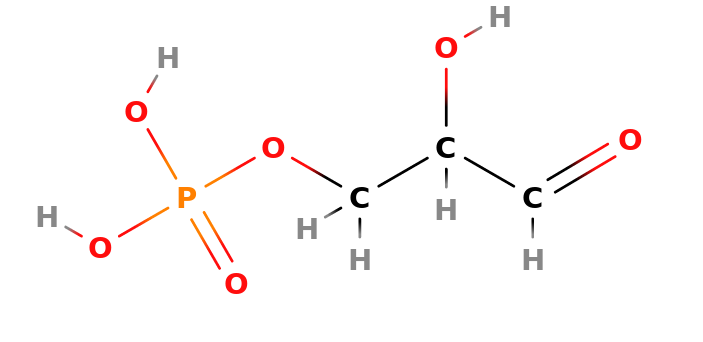
\includegraphics[width=0.8\linewidth]{g3p.png}
    \caption{Glyceraldehyde-3 phosphate}
    \label{fig: g3p}
\end{figure}

The effective chemical equation of photosynthesis is:

\ce{6CO2 + 6H2O ->[Sunlight] C6H12O6 + 6O2}

But note that there are several steps involved in this transformation.

\paragraph{Basic Photosynthetic Structures}
\begin{enumerate}
    \item In plants, it generally takes place in \emph{leaves} which have several layers of cells. The layer for photosynthesis is called \emph{mesophyll} (Greek: \emph{meso}: in the middle, \emph{-phyll}: leaf or pigment)
    \item The gas exchange takes place through \emph{stomata} (Greek: \emph{stoma}: mouth or opening)
\end{enumerate}

\subsection{Cell Communication}
\subsubsection{Signaling Molecules and Cellular Receptors}
\paragraph{Introduction}
In order to respond properly to external stimuli, cells have developed \emph{sophisticated} mechanisms of communication that can
\begin{enumerate}
    \item receive a \emph{message},
    \item transfer the information across the plasma membrane, and
    \item produce changes in the cell as a response
\end{enumerate}
Both single-celled (yes, single-celled) and multicellular organisms communicate with each other at a cellular level and across the organisms.

Communication within a cell is called the \emph{intracellular} communication, whereas the communication between two or more cells is called the \emph{intercellular} communication.

The small, usually volatile, and soluble signaling molecules that \emph{bind} to another specific molecule (and deliver a signal in the process) are called \emph{ligands}.

Ligands bind or interact with proteins called the \emph{receptor proteins} in the \emph{target cells} (the cells that would be affected by the ``signals''). Specific ligands bind with specific receptors. 

\subsection{Cell Reproduction}
\subsubsection{Introduction}
\textbf{A human, like every sexually reproducing organism, begins life as a fertilized egg (embryo) or zygote}. All multicellular organisms use cell division (even after they are fully grown) for growth and maintenance and repair of cells and tissues. Cell division is \emph{regulated closely}. Unicellular organisms also use cell division for their reproduction. 

Not all cells in the human body can reproduce \emph{to repair tissues}. Most nerve cells, for example, are not capable of regeneration. This means that people who have damaged their nerve cells or nervous system are often left paralyzed\footnote{This may change because of research}.
\subsubsection{Cell Division}
The cell cycle is an orderly sequence of events. It describes the stages of a cell's life from the division of a single parent cell to the production of two new genetically identical daughter cells.
\paragraph{Genomic DNA}
A cell's DNA, packaged as a double-stranded DNA molecule, is called its \emph{genome}. 

\lettrine[lines=2]{I}{n prokaryotes}, the genome is composed of a single DNA molecule. It's found in an area called \emph{nucleoid}. Sometimes, smaller loops of DNA called \emph{plasmids} are also present. Prokaryotes exchange plasmids with other prokaryotes. \emph{Antibiotic resistance} may be developed in a bacteria colony as a result of plasmid exchange between a resistant donor and recipient cells.

\lettrine[lines=2]{I}{n eukaryotes}, the genome is composed of several \emph{double stranded} linear DNA molecules. Each species has a \emph{characteristic number} of chromosomes. Human somatic (body) cells have 46 chromosomes, whereas human gametes (sperm or egg cells) have 23 chromosomes each.

\textbf{Matched pairs of chromosomes in a diploid organism are called \underline{homologous chromosomes}}. Each copy of a homologous chromosome originates in a different parent. The individual homologous chromosome therefore is not identical to its copy. \textbf{Regions of chromosome are identified as genes}. Genes are the \emph{functional units} of chromosome and they determine the phenotypical (externally visible) characteristics of an individual by \emph{encoding specific proteins}. 

A location on a chromosome is called \textbf{locus} and a gene is said to be located at some locus. Since there are population variations, two different humans are more likely to have variations in the genes. Although we do not have the DNA sequence of each human, there are statistical models that determine the form or version of each gene. \textbf{Each form or version of a gene at a given locus is called an allele}.
\subsubsection{The Cell Cycle}
\subsubsection{Control of the Cell Cycle}
\subsubsection{Cancer and the Cell Cycle}
\subsubsection{Prokaryotic Cell Division}

\section{Unit 3: Genetics}
\subsection{Meiosis and Sexual Reproduction}
\paragraph{Introduction}
\lettrine[lines=3]{T}{he ability} to reproduce ``in kind'' (the offspring closely resembles the parent(s)) in a basic characteristics of all living things. The Dr. Seuss story ``Horton hatches the egg'', however lyrical and sentimental, is ascientific (that, of course, does not reduce its literary value).

Many unicellular organisms, such as yeast, and a few multicellular organisms, such as sponges, \textbf{can produce genetically identical clones of themselves through cell division}. However, many single-celled organisms and most multicellular organisms reproduce regularly using ``Sexual Reproduction'', a method requiring two parents. Sexual reproduction occurs through
\begin{enumerate}
    \item the \emph{production by each parent of a \textbf{haploid} cell each containing only half of the required genetic information} (meiosis), and
    \item the \emph{fusion of these two haploid cells to form a single, unique diploid cell with a complete set of genetic information} (fertilization of an egg).
\end{enumerate}
\emph{Variation} or \emph{Variability} is an important component of the \emph{evolutionary success} of species. A vast majority of eukaryotes use \textbf{meiosis} and \textbf{fertilization} to ``reproduce''. But like Yashiro et.al. have argued in \cite{yashiro-matsuura} the prevalence of sexual reproduction remains an enigma. \emph{Queens} of Asian termites can reproduce both sexually and asexually (asexual reproduction may be better termed ``cloning'') by a method known as \emph{parthenogenesis} (The prefix parthen- means virgin in greek; development of embryo from an unfertilized egg).

\subsubsection{The Process of Meiosis}
\paragraph{Introduction}
In \emph{mitosis} cells divide to grow, replace other cells, and \emph{reproduce asexually}. \textbf{Without mutation}, or \textbf{changes in the DNA}, the daughter cells produced by mitosis receive a set of genetic instructions that is identical to that of the parent cell. Because changes in genes drive both the unity and diversity of life, organisms without genetic variation cannot evolve through natural selection. Evolution occurs only because organisms have developed ways to vary their genetic material. This occurs through 
\begin{itemize}
    \item mutations in DNA, 
    \item recombination of genes during meiosis, and 
    \item meiosis followed by fertilization in sexually reproducing organisms.
\end{itemize}
Sexual reproduction requires that diploid (2n) organisms produce haploid (1n) cells through meiosis and that these haploid cells fuse to form new, diploid offspring. The \emph{union of these two haploid cells}, one from each parent, is \emph{fertilization}.

The eukaryotic DNA is contained in chromosomes, and chromosomes occur in \emph{homologous pairs} (homologues). At fertilization, the male parent contributes one member of each homologous pair to the offspring, and the female parent contributes the other. With the exception of the sex chromosomes, homologous chromosomes contain the same genes, but \emph{these genes can have different variations, called alleles}. (For example, you might have inherited an allele for brown eyes from your father and an allele for blue eyes from your mother.) As in mitosis, homologous chromosomes are duplicated during the S-stage (synthesis) of interphase. However, unlike mitosis, in which there is just one nuclear division, meiosis has two complete rounds of nuclear division—meiosis I and meiosis II. These result in four nuclei and (usually) four daughter cells, each with half the number of chromosomes as the parent cell (1n). The first division, meiosis I, separates homologous chromosomes, and the second division, meiosis II, separates chromatids. 


\ctext{white}{purple}{During meiosis, DNA replicates ONCE but divides TWICE, whereas in mitosis, DNA replicates ONCE but divides only ONCE.}

It is important to note that \cite{embryo-project} meiosis is the process by which sexually reproducing organisms generate gametes (sex cells). However, the main function of meiosis is \textbf{the reduction of the ploidy (number of chromosomes) of the gametes from diploid (2n, or two sets of 23 chromosomes) to haploid (1n or one set of 23 chromosomes)}.

Both males and females use meiosis to produce their gametes, although there are some key differences between the sexes at certain stages. In females, the process of meiosis is called \textbf{oogenesis}, since it produces oocytes and ultimately yields mature ova(eggs). The male counterpart is \textbf{spermatogenesis}, the production of sperm. While they occur at different times and different locations depending on the sex, both processes begin meiosis in essentially the same way. \textbf{Meiosis occurs in the primordial germ cells, cells specified for sexual reproduction and separate from the body’s normal somatic cells}  \cite{embryo-project}.

See Figure \ref{fig: meiosis-1} for some terminology.

\begin{figure}[h!]
    \centering
    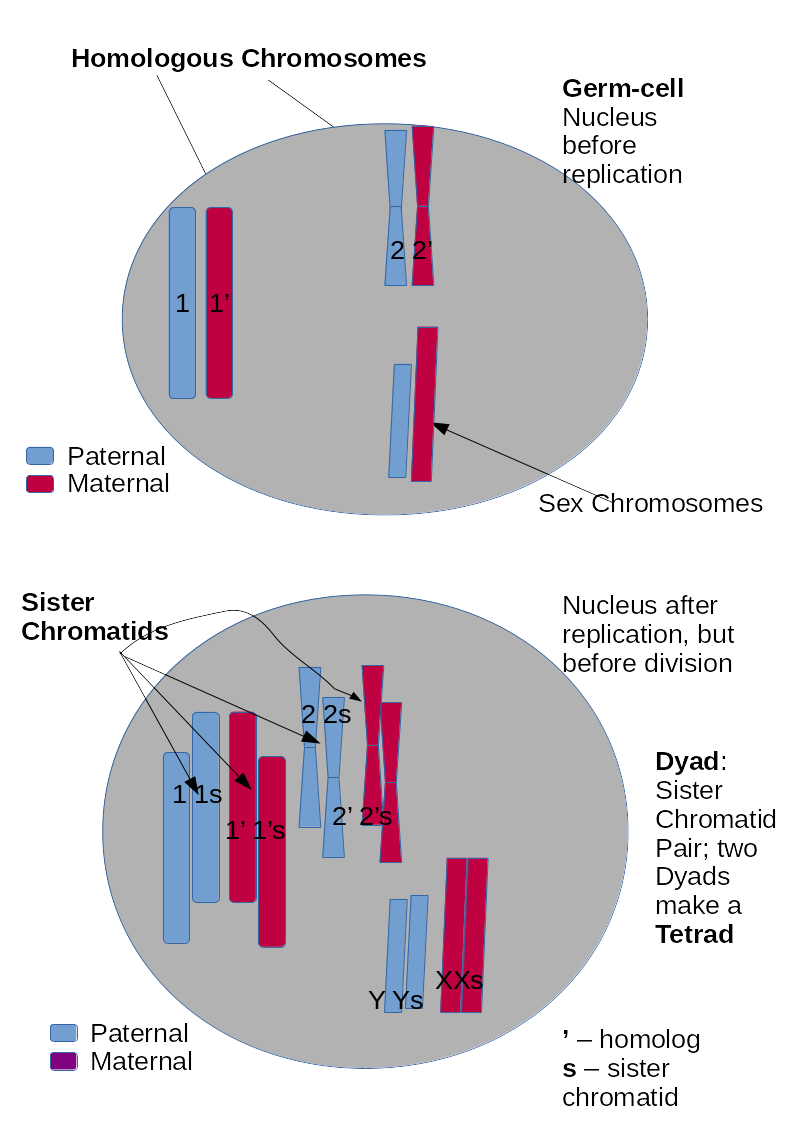
\includegraphics[scale=0.3]{meiosis-1.png}
    \caption{Meiosis terminology for a germ cell}
    \label{fig: meiosis-1}
\end{figure}

\newpage

The \href{https://upload.wikimedia.org/wikipedia/commons/7/74/Meiosis_Stages.svg}{Wikipedia page} has many good figures and explanation of meiosis. It is important to realize that the \textbf{germ cells that undergo meiosis are different from the sperm and egg cells}. Germ cells are diploid (2n) cells. 

Meiosis proceeds in two distinct stages called Meiosis I and Meiosis II.

\textbf{Steps in Meiosis I}:
\begin{enumerate}
    \item \textbf{Prophase I}. Mitosis preceeds meiosis. A germ cell divides by mitosis. Figure shows the \textbf{diploid} oogonium (egg cell) or spermatogonium (sperm). This is the Prophase I. At this stage, as you can see, there are sister chromatids for each chromosome (including the X- and the Y-chromosome). 
\begin{figure}[h!]
    \centering
    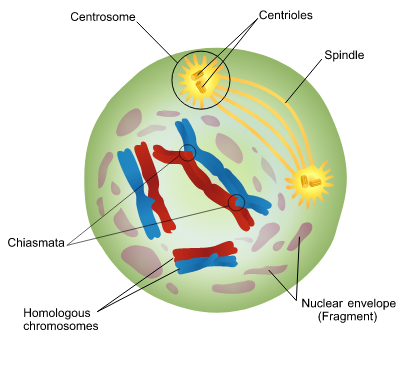
\includegraphics[scale=0.4]{prophase-I.png}
    \caption{Prophase-I: chromosomes condense and crossover begings to happen}
    \label{fig: prophase-I}
\end{figure}
        The synapse formation is shown below. Note the difference between homologous chromosomes and sister chromatids. Figure \ref{fig: synapse-formation} shows the replication of the genetic material in the diploid cell. 
\begin{figure}[h!]
    \centering
    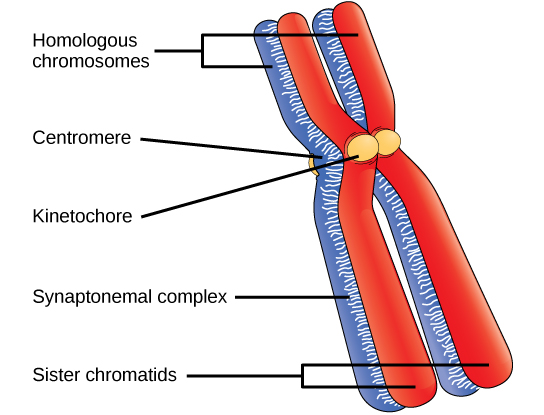
\includegraphics[scale=0.4]{synapse-formation.jpeg}
    \caption{Prophase-I: Synaptonemal complex, centromere, and synapse formation}
    \label{fig: synapse-formation}
\end{figure}
        Located at intervals along the synaptonemal complex are large protein assemblies called \textbf{recombination nodules}. These assemblies mark the points of later chiasmata and mediate the multistep process of \emph{crossover}—or \emph{genetic recombination}—between the \emph{non-sister chromatids}. Near the recombination nodule on each chromatid, the double-stranded DNA is cleaved, the cut ends are modified, and \textbf{a new connection is made between the non-sister chromatids}. A chiasma (pl. chiasmata) is the point of contact, the physical link, between two (non-sister) chromatids belonging to homologous chromosomes. At a given chiasma, an exchange of genetic material (a \emph{chromosomal crossover}) can occur between both chromatids, but this is much \href{https://en.wikipedia.org/wiki/Chiasma_(genetics)}{more frequent during meiosis than mitosis}. In meiosis, absence of a chiasma generally results in improper chromosomal segregation and \textbf{aneuploidy} (presence of an abnormal number of chromosomes in a cell, for example a human cell having 45 or 47 chromosomes instead of the usual 46.)

        At the end of prophase I, the pairs are held together only at the chiasmata (Figure \ref{fig: crossover-in-action}) and are called tetrads because the four sister chromatids of each pair of homologous chromosomes are now visible.

\begin{figure}[h!]
    \centering
    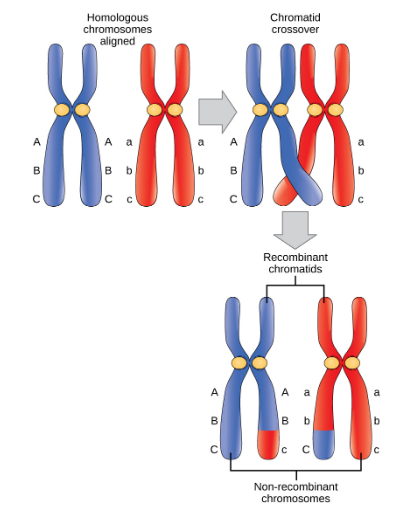
\includegraphics[scale=0.4]{crossover-in-action.png}
    \caption{Prophase I: Crossover in action}
    \label{fig: crossover-in-action}
\end{figure}
        \textbf{The crossover events are the first source of genetic variation in the nuclei produced by meiosis}. A single crossover event between homologous non-sister chromatids leads to a reciprocal exchange of equivalent DNA between a maternal chromosome and a paternal chromosome. Now, when that sister chromatid is moved into a gamete cell it will carry some DNA from one parent of the individual and some DNA from the other parent. \textbf{The sister recombinant chromatid has a combination of maternal and paternal genes that did not exist before the crossover}. Multiple crossovers in an arm of the chromosome have the same effect, exchanging segments of DNA to create recombinant chromosomes.

    \item \textbf{Metaphase I}. During metaphase I, the homologous chromosomes are arranged in the center of the cell with the kinetochores facing opposite poles. The homologous pairs orient themselves \emph{randomly} at the equator. 
\begin{figure}[h!]
    \centering
    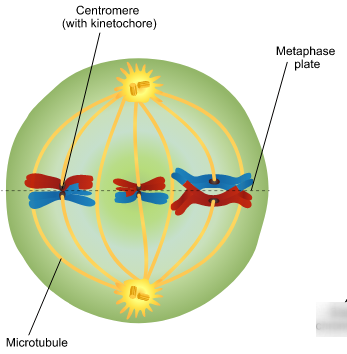
\includegraphics[scale=0.4]{metaphase-I.png}
    \caption{Metaphase I: Chromosome pairs move to the equator of the cell}
    \label{fig: metaphase-I}
\end{figure}
        \textbf{The crossover events are the first source of genetic variation in the nuclei produced by meiosis}. A single crossover event between homologous non-sister chromatids leads to a reciprocal exchange of equivalent DNA between a maternal chromosome and a paternal chromosome. Now, when that sister chromatid is moved into a gamete cell it will carry some DNA from one parent of the individual and some DNA from the other parent. \textbf{The sister recombinant chromatid has a combination of maternal and paternal genes that did not exist before the crossover}. Multiple crossovers in an arm of the chromosome have the same effect, exchanging segments of DNA to create recombinant chromosomes.
\end{enumerate}


\newpage
\subsection{Mendel's Experiments and Heredity}

\subsubsection{Mendel's Experiments and the Laws of Probability}
Johann Gregor Mendel conducted experiments to demonstrate the existence of genes long before the term was coined. His experiments are an exemplary lesson in the ``design and execution of scientific experiments''. Mendel is regarded as the father of modern genetics.

\subsubsection{Extra: Mendel's Experiments (Refers to Various Resources)}
Mendel wanted to investigate if there was a \emph{general law} for the formation and development of \emph{hybrids}, something he noted had not been previously formulated \cite{mendel-fisher}: 
\epigraph{
    Those who survey the work done in this department will arrive at the conviction that among all the numerous experiments made, \emph{not one has been carried out to such an extent and in such a way as to make it possible to determine the number of different forms under which the offspring of hybrids appear}, or to arrange these forms with certainty according to their separate generations, or definitely to ascertain their statistical relations.
}
{
    ---\textit{Johann Gregor Mendel \cite{mendel-fisher}}
}

Mendel and his colleagues carried out their experiments for nearly a decade (1856-1865). Mendel required \cite{mendel-fisher} that the experimental plant must
\begin{enumerate}
    \item possess constant differentiating factors
    \item be capable, during flowering, of protecting from the influence of \emph{foreign pollen}
\end{enumerate}

After careful analysis of various options, Mendel chose ``garden pea'' (\emph{Pisum Sativum L.}) to experiment with. He decided to experiment with the garden pea and examine following traits:
\begin{enumerate}
    \item Seed shape: Round or Wrinkled (a \emph{seed\footnote{A characteristic that can be ascertained by simply analyzing the seed}} characteristic)
    \item Cotyledon (the first leaves that sprout out of the seed upon germination) color: Yellow or Green (a seed characteristic)
    \item Seed-coat color: Colored or White (a \emph{plant\footnote{A characteristic that can only be ascertained by waiting for a plant to grow from the seed} characteristic})
    \item Pod shape: Inflated or Constricted (a plant characteristic)
    \item Pod color: Green or Yellow (a plant characteristic)
    \item Flower position: Axial (along the stem) or Terminal (at the end of the stem) (a plant characteristic)
    \item Stem length: Long (6--7 feet) or Short (less than a foot) (a plant characteristic)
\end{enumerate}

An interesting and somewhat philosophical question arises: ``Chicken first or egg first?'' Mendel tried to answer it from what he had available: Generations of ``true-bred'' plants which were available in the monastery garden where he conducted the experiments. 

There is a lot of terminology here and we need to understand just what the \emph{key terms} mean before proceeding. We should also put ourselves into Mendel's shoes and try to reason the way he did. Explaining what Mendel did using the modern Genetics terms is likely to be confusing. For example, we shouldn't be using a term like \emph{homozygous} because Mendel didn't even know what that term meant. Of course, at some point we should reconcile all of this in terms of contemporary knowledge. 

Note that a seed belongs to the generation of the plant that comes \emph{after} the [generation of the] plant whose fruit bears the seeds.

Here are the key terms in the order of their dependence (i.e. a term appearing later in the list will depend on the terms appearing before):
\begin{enumerate}
    \item \textbf{Character}: This is a heritable feature, for example, stem length. Typically, an organism simultaneously exhibits several different Characters.
    \item \textbf{Trait}: Each \emph{variant} of a Character is called a Trait, for example, a plant could have ``Tall'' (stem length) Trait.
    \item \textbf{True-bred}: This is an adjective (past participle of ``True-breed''), typically applied to an organism. An organism is said to be True-bred from seed alone with respect to certain Traits when it passes down those Traits to its offspring (more generally, descendants) \emph{of many generations}. Since flowering plants have both female and male reproductive organs, true-bred Traits of many plants can be created by their \emph{self-pollination}. (Note, however, that flowering plants like apple are notorious for not breeding true from seed; apple needs to be \emph{grafted}). Mendel started with true-bred pea plants mainly because they were relatively much easier to true-breed from seed by self-pollination.
    \item \textbf{Cross}: Fertilization of the egg by the pollen from another plant. Since a single flowering plant has, unlike humans, both male and female reproductive organs, Mendel had to prevent their self-pollination in order to carry out the desired crosses. In a way, a cross-bred offspring is opposite of a true-bred offspring.
    \item \textbf{Monohybrid Cross}: Cross between two \emph{true-bred} organisms of a species that differ in a single Trait. Mendel painstakingly carried out such crosses with peas (e.g. by crossing true-bred green-seed plants with true-bred yellow-seed plants).
    \item \textbf{Dominance}: The ability of a certain Trait (of a given Characteristic) to express in 
    \item \textbf{Submissiveness}:
\end{enumerate}

\subsubsection{Characteristics and Traits}
\subsubsection{Laws of Inheritance}

\subsection{Modern Understandings of Inheritance}
\subsection{DNA Structure and Function}
\textbf{Each person’s DNA is unique, and it is possible to detect differences among individuals within a species on the basis of these unique features}. DNA analysis has many practical applications, including identifying criminals (forensics), determining paternity, tracing genealogy, identifying pathogens, researching archeological finds, tracing disease outbreaks, and studying human migration patterns. In the medical field, DNA is used in diagnostics, new vaccine development, and cancer therapy. It is often possible to determine predisposition to diseases by sequencing genes.

Sometimes an innocent person is erroneously convicted of a crime and sent to jail. Between 2000 and 2015, evidence from DNA was used to exonerate over 250 innocent people. Twenty of those people were on death row after being convicted of a murder they didn’t commit. To learn more about the intense scientific and legal processes used to exonerate those wrongfully convicted, go to The Innocence Project website \href{http://www.openstax.org/l/32innocence}{here}.
\subsubsection{Historical Basis of Modern Understanding}

\subsection{Genes and Proteins}
\subsection{Gene Regulation}
\subsection{Biotechnology and Genomics}

\section{Unit 4: Evolution}
\subsection{Evolution and Origin of Species}
\paragraph{Introduction}
Evolution is an all-pervasive idea in biology. Even so, teaching, in public schools, evolution as science is debated. 
\epigraph{
    Nothing in Biology Makes Sense \\
    Except in the Light of Evolution.
}{
    \textit{Theodosius Dobzhansky \cite{light-of-evol}}
}
\par\bigskip
There are not many topics in the history of thought on which humans are as divided as they are on the idea of evolution. To understand, in scientific and non-scientific contexts, topics as fundamental, diverse, fascinating, and complex as evolution and the origin of species, we need to first \emph{clearly} define the words we often use casually. Be warned, however, that defining terms clearly is quite challenging! Using a word or term to mean two different things is called ``overloading a term". Overloading happens a lot, especially across contexts. Therefore, we should not take sentences, quotations etc. out of context. The terms are defined here in a scientific context. I am deliberately leaving out of scope what ``scientific" means, but simply put, it means anything that is \emph{falsifiable}; everything in science, unlike religion, is open to be proved false by providing evidence that can be verified by various different means and people.
\par\bigskip

\emph{Sincere search and probable determination of truth} is what science promotes. Since the universe is extremely complex and the devil is in the detail, determination of truth of even an \emph{isolated system} remains illusive. As we progress, advances are made, we know more and either previous claims are strengthened or falsified (Wikipedia \cite{superseded} gives a detailed list of superceded theories.) Dobzhansky's paper \cite{light-of-evol} is a great \emph{position statement} on how to keep scientific endeavor and personal beliefs separate.
\par\bigskip

Let's try to define some common terms and use them consistently (or hope that they have been used consistently) in a scientific context (See \cite{teaching-evol}) throughout this text. This is not a comprehensive list of terms:
\begin{itemize}
    \item \textbf{Fact}: An observation that is \emph{repeatedly confirmed} by uniformly calibrated measuring tools and by different people. Objectivity of what one is experiencing is key here. You don't bring in your emotions to decide whether something is a \emph{fact}. We need to take into account human flaw named \emph{confirmation bias}, but when some observation is made or confirmed by many observers, we expect it to be free of any bias. It is futile to deny facts. Examples: Earth is round, rolling friction is smaller than sliding friction, oil is lighter than water, a ball of metal sinks in water while a much heavier ship floats, solar eclipse happens during the daytime and lunar eclipse happens at night, every celestial body appears to rise in the east and sets in the west, a ball rolls down the slope by itself while it needs to be pushed up the slope etc.
    \item \textbf{Hypothesis}: A \emph{testable} statement that can be used to explain more complex aspect of or process in the natural world. It is usually a logical guess made while answering a question or explaining a behavior or observation. A hypothesis may provide a probable research direction.
    \item \textbf{Law}: 
\end{itemize}

\subsubsection{Understanding Evolution}
\subsubsection{Formation of New Species}
\subsubsection{Reconnection and Rates of Speciation}


\subsection{Evolution of Populations}
\paragraph{Introduction}
\subsubsection{Population Evolution}
\subsubsection{Population Genetics}
\subsubsection{Adaptive Evolution}

\section{Unit 5: Viruses}

\section{Unit 23: Plant Form and Physiology}
\paragraph{Introduction}
\subsection{The Plant Body}
\subsection{Stems}
\subsection{Roots}
\subsection{Leaves}
\subsection{Transport of Water and Solutes in Plants}

\begin{thebibliography}{00}
    \bibitem{mendel-fisher} Allan Franklin, A. W. F. Edwards, Daniel J. Fairbanks, Daniel L. Hartl. Ending the Fisher-Mendel Controversy. University of Pittsburgh Press, 2008. Page 2.

    \bibitem{yashiro-matsuura} Yashiro, Toshihisa and Matsuura, Kenji. (2014). Termite queens close the sperm gates of eggs to switch from sexual to asexual reproduction. Proceedings of the National Academy of Sciences. 111. 17212-17217. 10.1073/pnas.1412481111. 

    \bibitem{embryo-project} Maayan, Inbar. ``\href{http://embryo.asu.edu/handle/10776/2084}{Meiosis in Humans}''. Embryo Project Encyclopedia (2011-03-24). ISSN: 1940-5030. 

    \bibitem{meiosis-int-demo} \href{https://www.cellsalive.com/meiosis_js.htm}{Animal Cell Meiosis}.

    \bibitem{the-central-dogma} Crick Francis. ``On Protein Synthesis". \href{https://libgallery.cshl.edu}{CSHL Archives Repository}.

    \bibitem{mallery} Mallery Charles. \href{http://henge.bio.miami.edu/mallery/150/}{Biology 150 and Biology 255}.
        
    \bibitem{ih-mh} Istav{\'a}n Hargittai, Magdolna Hargittai. Candid Science VI: More Conversations With Famous Scientists. Imperial College Press. 2006. ISBN 1-86094-694-1.

    \bibitem{koonin} Eugene V. Koonin. ``Does the central dogma still stand?" \href{https://biologydirect.biomedcentral.com/articles/10.1186/1745-6150-7-27}{Biology Direct}. 23 August 2012. 
        
    \bibitem{alphafold} AlphaFold: Using AI for Scientific Discovery. \href{https://deepmind.com/blog/article/AlphaFold-Using-AI-for-scientific-discovery}{DeepMind}.

    \bibitem{light-of-evol} Thodosius Dobzhansky. Nothing in Biology Makes Sense Except in the Light of Evolution. The American Biology Teacher, Vol. 35, No. 3 (March 1973), pp. 125-129.
        
    \bibitem{teaching-evol} Teaching About Evolution and the Nature of Science. Working Group on Teaching Evolution, National Academy of Science. \href{http://nap.edu/5787}{PDF}.

    \bibitem{superseded} Wikipedia. \href{https://en.wikipedia.org/wiki/Superseded_theories_in_science}{Superseded Theories in Science}.
\end{thebibliography}
\end{document}
